\documentclass[xcolor=table, aspectratio=169,ignorenonframetext]{beamer}

%\documentclass{article}
%\usepackage{beamerarticle}

%\usepackage{arev}
\usepackage{amsmath,amssymb,amscd}
\usepackage{dsfont}
\usepackage{mathrsfs}
\usepackage{yfonts}
\usepackage{bm}
\usepackage{graphicx}
\usepackage{tabularx}
\usepackage{animate}
%\usepackage{ifthen}

%\usepackage{xeCJK}
%\usepackage{fontspec}
%\newfontfamily\cjkfont{PingFang SC}
%\setCJKmainfont{PingFang SC}
\newcolumntype{x}{>{\centering\arraybackslash}X}
\renewcommand{\arraystretch}{1.5}
\DeclareMathOperator{\img}{img}
\DeclareMathOperator{\hhom}{Hom}
\newcommand{\uone}{\text U(1)}

\usepackage{tikz}
	\usetikzlibrary{calc}
	\usetikzlibrary{arrows,shapes, positioning, matrix}
	\usetikzlibrary{decorations.markings}
	\tikzstyle arrowstyle=[scale=1]
  \tikzstyle string=[thick,postaction={decorate,decoration={markings,
      mark=at position .55 with {\arrow[arrowstyle]{stealth}}}}]

\usepackage{pgffor}
\newcommand{\cohosub}[1]{\scalebox{0.72}{\textswab{#1}}}
\newcommand{\cohosubsub}[1]{\scalebox{0.6}{\textswab{#1}}}
\newcommand{\coho}[1]{\textswab{#1}}


\mode<presentation>
{
  %\usetheme{Warsaw}
  % or ...
  %\useoutertheme{rectangle}
  \setbeamertemplate{frametitle}[default][center]
  \defbeamertemplate{itemize item}{flat}{\begin{pgfpicture}{-1ex}{0ex}{1ex}{2ex}
      \pgfpathcircle{\pgfpoint{0pt}{.6ex}}{0.6ex}
      \pgfusepath{fill}
    \end{pgfpicture}%
  }
  \defbeamertemplate{itemize subitem}{flat}{\footnotesize\raise0.5pt\hbox{\textbullet}}
  \defbeamertemplate{itemize subsubitem}{flat}{\footnotesize\raise0.5pt\hbox{\textbullet}}

  %\useinnertheme{circles}
  \setbeamertemplate{items}[flat]
  \setbeamertemplate{sections/subsections in toc}[circle]
  \setbeamertemplate{blocks}[rounded]
  \setbeamertemplate{title page}[default][colsep=-4bp,rounded=true]
  \setbeamertemplate{part page}[default][colsep=-4bp,rounded=true]
  \setbeamercovered{transparent}
  %\usecolortheme{spruce}
  %\definecolor{THU}{RGB}{116,61,130}
  \definecolor{mbg}{RGB}{0,0,160}
  \setbeamercolor*{palette primary}{fg=white,bg=mbg}
  \setbeamercolor*{titlelike}{parent=palette primary}
  \setbeamercolor*{structure}{fg=mbg}
  \setbeamercolor{frametitle}{fg=white,bg=mbg}
  % or whatever (possibly just delete it)
  \setbeamercolor{block title}{bg=mbg,fg=white}
  \setbeamercolor{block body}{bg=mbg!15}


  \addtobeamertemplate{navigation symbols}{}{ \hspace{1em}%
    \usebeamerfont{footline}%
    \insertframenumber / \inserttotalframenumber }
}


%\usepackage[english]{babel}
% or whatever

%\usepackage[latin1]{inputenc}
% or whatever

%\usepackage{times}
%\usepackage[T1]{fontenc}
% Or whatever. Note that the encoding and the font should match. If T1
% does not look nice, try deleting the line with the fontenc.

\title % (optional, use only with long paper titles)
{Lecture 1: SPT phases and cohomology theory}
\author[Y Qi] % (optional, use only with lots of authors)
{Yang~Qi}
% - Give the names in the same order as the appear in the paper.
% - Use the \inst{?} command only if the authors have different
%   affiliation.

\institute[Fudan] % (optional, but mostly needed)
{
Department of Physics, Fudan University.
}
% - Use the \inst command only if there are several affiliations.
% - Keep it simple, no one is interested in your street address.

%\date{2016 Annual Meeting of Fudan CFTPP} % (optional, should be abbreviation of conference name)
%{Fudan University, Oct 13 2015}
\date{Nov. 29-30, 2019}
% - Either use conference name or its abbreviation.
% - Not really informative to the audience, more for people (including
%   yourself) who are reading the slides online

%\subject{Theoretical Physics}
% This is only inserted into the PDF information catalog. Can be left
% out.



% If you have a file called "university-logo-filename.xxx", where xxx
% is a graphic format that can be processed by latex or pdflatex,
% resp., then you can add a logo as follows:

\pgfdeclareimage[height=1cm]{university-logo}{../resources/fudan}
\logo{\pgfuseimage{university-logo}}



% Delete this, if you do not want the table of contents to pop up at
% the beginning of each subsection:
\AtBeginSection[]
{
  \begin{frame}<beamer>{Outline}
			\tableofcontents[currentsection,currentsubsection]
  \end{frame}
}
%\AtBeginSubsection[]
%{
 % \begin{frame}<beamer>{Outline}
  %  \tableofcontents[currentsection,currentsubsection]
  %\end{frame}
%}


\begin{document}

\begin{frame}
  \titlepage
\end{frame}

\begin{frame}{Outline}
	%\begin{columns}
	%\column{.7\textwidth}
		\tableofcontents
  %\end{columns}
  % You might wish to add the option [pausesections]
\end{frame}

\section{Introduction: What are SPT states}

\begin{frame}
  \frametitle{Symmetry-Protected Topological (SPT) states}
\begin{itemize}
\item SPT: gapped topological phases beyond Landau paradiam.
\item Cannot be smoothly connected to a trivial state without closing gap or breaking symmetry.
\item Symmetry-protected gapless surface states.
\item Free-fermion states: topological insulators, topological superconductors.
\item Bosonic SPTs: Haldane chain, CZX/Levin-Gu state, etc.\\
\emph{Xie Chen, Zheng-Cheng Gu, Zheng-Xin Liu and Xiao-Gang Wen, Science 2012.}
\item Interacting fermionic SPTs.
\end{itemize}
\end{frame}

\begin{frame}
	\frametitle{Abelian-group classification}
	\begin{itemize}
		\item SPT phases and boundary anomalies are classified by Abelian groups ($\mathbb Z$ or $\mathbb Z_n$).
		\begin{itemize}
			\item Addition: stacking of phases/gapless boundaries.
			\item 0: The trivial phase/gapped boundary.
		\end{itemize}
		\item 2D Chern-insulators (Integer Quantum Hall):
		\begin{center}
				\includegraphics[width=8cm]{../spspt/qhe_edge}
		\end{center}
		Classified by $\mathbb Z$: $[n]+[m]=[n+m]$; $[n]+[-n] = 0$.
	\end{itemize}
\end{frame}

\begin{frame}
	\frametitle{Abelian-group classification}
	\begin{itemize}
		\item 3D Topological Insulators:
		\begin{center}
			\includegraphics[width=8cm]{../spspt/ti_surface}
		\end{center}
		Classified by $\mathbb Z_2$: $[1]+[1] = 0$.
		\item 1D Haldane chain:
		\begin{center}
			\includegraphics[width=6cm]{../dimer/weak3d_aklt_blue}
		\end{center}
		Classified by $\mathbb Z_2$: $[1]+[1] = 0$.
	\end{itemize}
\end{frame}

\section{Constructing an SPT state}

\begin{frame}
\frametitle{Group-cohomology model}
\begin{itemize}
\item Consider an onsite symmetry group $G$, $|G|<\infty$.
\item A space-time $\Delta$-lattice: $d+1$-simplexes (triangles, tetrahedra, etc).
\item Branching structure: an ordering $1>2>\cdots>N$; an orientation $i\rightarrow j$ if $i<j$.
\item Hilbert space: $\otimes_i |g_i\rangle$, $g_i\in G$.
\item Symmetry transformation:
$g|g_i\rangle = |gg_i\rangle$.
\end{itemize}
\begin{center}
\includegraphics[height=3cm]{tri-lattice}
\end{center}
\end{frame}

\begin{frame}
\frametitle{Partition function}
\[Z = \sum_{\{g_i\}}e^{iS},\quad
S = \sum_{\Delta ijk}2\pi s_{ijk}\omega(g_i,g_j,g_k).\]

\begin{center}
\includegraphics[height=4cm]{tri-orient}
\end{center}

Function $\omega:G\times G\times\cdots\times G\rightarrow \mathbb R/\mathbb Z$.
\end{frame}

\begin{frame}
\frametitle{Symmetry condition}

\begin{itemize}
\item $G$ action:
$\omega(g_0, \ldots, g_{d+1})\rightarrow \omega(gg_1, \ldots, gg_{d+1})$.
\item If $g$ is unitary: $S$ should be invariant. $\omega(g_0, \ldots, g_{d+1})= \omega(gg_0, \ldots, gg_{d+1})$.

\item $g$ is antiunitary: $S\rightarrow -S$. $\omega(g_0, \ldots, g_{d+1})= -\omega(gg_0, \ldots, gg_{d+1})$.
\item $s(g)=\pm1$ if g is unitary/antiunitary.
\item $G$-action on $\mathbb R/\mathbb Z$:
$g\cdot x=s(g)x$.
\item Homogeneous condition:
\[g\cdot\omega(g_0, \ldots, g_{d+1})= \omega(gg_0, \ldots, gg_{d+1})\]
\end{itemize}

\begin{center}
\includegraphics[height=2.5cm]{tri-action}
\end{center}
\end{frame}

\begin{frame}
\frametitle{Fixed-point properties: invariant under RG}
\begin{itemize}
\item SPT phases are gapped phases.
\item Gapped phases are stable fixed points in RG flow diagrams, with $\xi=0$.
\item Invariant under scale transformation.
\item Discrete version of scale transformation: re-triangularization.
\end{itemize}

\begin{center}
	\includegraphics[height=4cm]{RGflow}
	\hspace{1cm}
	\includegraphics[height=4cm]{retri1}
\end{center}
\end{frame}

\begin{frame}
\frametitle{Cocycle conditions}
\begin{itemize}
	\item 3-1 move:
	$\omega(g_0,g_1,g_2) = \omega(g_0,g_1,g_3)
	-\omega(g_0,g_2,g_3) + \omega(g_1,g_2,g_3)$.
	\item 2-2 move:
	$\omega(g_0,g_1,g_2)-\omega(g_1, g_2,g_3)
	=\omega(g_0, g_1, g_3) - \omega(g_0, g_2, g_3)$.
	\item Cocycle equation:
	$d\omega(g_0,g_1,g_2,g_3)=\omega(g_1,g_2,g_3)
	-\omega(g_0,g_2,g_3)+\omega(g_0,g_1,g_3)-\omega(g_0,g_1,g_2)=0$.
\end{itemize}
\begin{center}
	\includegraphics[height=4cm]{moves}
\end{center}
\end{frame}

\begin{frame}
\frametitle{Gauge transformation: coboundary equivalence}
\begin{itemize}
	\item A coboundary $\omega(012)=d\mu(012)=\mu(12)-\mu(02)+\mu(01)$.
	\item On a \alert{closed} manifold:
	\item $\omega$ and $\omega + d\mu$ gives the same partition function.
	\item $\omega\sim\omega + d\mu$.
\end{itemize}
\begin{center}
\includegraphics[height=4cm]{tri-orient}
\end{center}
\end{frame}

\begin{frame}
\frametitle{Formal definition: group cohomology}
\begin{itemize}
	\item $n$-cochain $\omega: G^{\times n+1}\rightarrow \text{U}(1)$, satisfying homogeneous condition
	\[g\cdot\omega(g_0,\ldots,g_n) = \omega(gg_0,\ldots,gg_n).\]
	We denote the space of $n$-cochains by $C^n[G,\text U(1)]$.
	\item Define a coboundary operation $d^n:C^n[G,\text U(1)]\rightarrow C^{n+1}[G,\text U(1)]$
	\[d\omega(g_0,\ldots,g_{n+1})=\sum_{i=0}^n(-1)^n\omega(g_0,\ldots,\hat g_i,\ldots,g_n).\]
	\item This forms a cochain complex:
	\[C^0\xrightarrow{d^0}C^1\rightarrow\cdots\rightarrow C^{n-1}\xrightarrow{d^{n-1}}C^n\xrightarrow{d^n}C^{n+1}\rightarrow\cdots\]
\end{itemize}
\end{frame}

\begin{frame}
	\frametitle{Formal definition: group cohomology}
	\begin{itemize}
		\item The cochain complex:
		\[C^0\xrightarrow{d^0}C^1\rightarrow\cdots\rightarrow C^{n-1}\xrightarrow{d^{n-1}}C^n\xrightarrow{d^n}C^{n+1}\rightarrow\cdots\]
		satisfying $d^2=0$ ($d^n\circ d^{n-1}=0$)
		\item We can define cohomology groups:
		\[H^n[G,\text U(1)] = \frac{Z^n}{B^n} = \frac{\ker d^n}{\img d^{n-1}}.\]
		\item $(d+1)$-dimensional fixed-point partition functions are given by
		\[H^{d+1}[G,\text U(1)].\]
	\end{itemize}
\end{frame}

\section{Detecting an SPT state}

\begin{frame}
	\frametitle{Cannot detect from the bulk}
	\begin{itemize}
		\item Symmetry-breaking phases: detecting long-range order / Goldstone mode.
		\item SPT: Bulk is gapped and have trivial excitations.
		\item Edge states.
		\item Symmetry twist: Laughlin's argument.
	\end{itemize}
	\begin{center}
		%\includegraphics[height=4cm]{ti_band}
	\end{center}
\end{frame}

\begin{frame}
	\frametitle{Laughlin's argument}
	\begin{itemize}
		\item Threading a $2\pi$ flux ($\Phi_0 = hc/e$) through the hole of a cylinder.
		\item $\Phi(t)\Rightarrow E_y\Rightarrow I_x$.
		\item $ne$-charge is transported across the system.
	\end{itemize}
	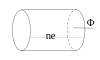
\includegraphics{laughlin}
\end{frame}

\begin{frame}
	\frametitle{Symmetry twist: a global static gauge flux}
	\begin{columns}
		\column{.35\textwidth}
		\begin{itemize}
			\item U(1) symmetry\\
			$c_i^\dagger c_j\rightarrow e^{i\theta}c_i^\dagger c_j$;\\
			$c_i\rightarrow c_ie^{i\theta}$.
			\item $\mathbb Z_2$ symmetry\\
			$s_is_j\rightarrow-s_is_j$;\\
			$s_i\rightarrow -s_i$.
		\end{itemize}
		\column{.65\textwidth}
		\includegraphics<1>{sym-twist}
		\includegraphics<2>{sym-gauge}
	\end{columns}
\end{frame}

\begin{frame}
	\frametitle{Partition function of SPT state}
	\begin{itemize}
		\item Considier a finite, unitary symmetry group $G$.
		\item Take a $(d+1)$-dimensional space-time manifold $M$,
		\item And $\gamma:\pi_1(M)\rightarrow G$,
		\item An SPT phase: a partition function $Z(M,\gamma)$.\\
		\emph{$M$ and $\gamma$ forms a $G$-bundle}.
	\end{itemize}
	\begin{center}
		\includegraphics[height=3cm]{manifold}
	\end{center}
	{\small Dijkgraaf and Witten, Comm. Math. Phys. \textbf{129} 393 (1990).}
\end{frame}

\begin{frame}
	\frametitle{Universal bundle}
	\begin{itemize}
		\item Universal bundle: $p: EG \rightarrow BG$.
		\item Classifying space: $BG$ satisfying\\
		$\pi_1(BG) = G$, $\pi_2(BG)=0$, $\pi_3(BG)=0$, ...
		\item $\gamma:\pi_1(M)\rightarrow G=\pi_1(BG)$ can be extended to $\gamma:M\rightarrow BG$.
	\end{itemize}
\end{frame}

\begin{frame}
	\frametitle{Cohomology groups of $BG$}
	\begin{itemize}
		\item Realize $BG$ as a CW-complex.
		\item A chain complex
		\[C_n(BG)\xrightarrow{\partial_n}
		C_{n-1}(BG)\rightarrow\cdots\rightarrow
		C_1(BG)\xrightarrow{\partial_1}
		C_0(BG)\xrightarrow{\epsilon}\mathbb Z\rightarrow0.\]
		\item $\partial^2=0$
		\item Define cochain space $C^n=\hhom[C_n,\text U(1)]$, $d = \partial^\ast$.
		\item A cochain complex
		\[C^0\xrightarrow{d^0}C^1\rightarrow\cdots\rightarrow C^{n-1}\xrightarrow{d^{n-1}}C^n\xrightarrow{d^n}C^{n+1}\rightarrow\cdots\]
		satisfying $d^2=0$ ($d^n\circ d^{n-1}=0$)
		\item We can define cohomology groups:
		\[H^n[BG,\text U(1)] = \frac{Z^n}{B^n} = \frac{\ker d^n}{\img d^{n-1}}.\]
	\end{itemize}
\end{frame}

\begin{frame}
	\frametitle{Partition function on a $G$-bundle}
	\begin{itemize}
		\item Given space-time orientable manifold $M$ and $\gamma:M\rightarrow BG$.
		\item Take a cochain $\alpha$
		\item Pullback map: $\gamma^\ast\alpha$ is a cochain on $M$.
		\[\langle \gamma^\ast\alpha, x\rangle = \langle \alpha,\gamma(x)\rangle.\]
		\item We can construct $Z$:
		\[Z = \langle\gamma^\ast\alpha, [M]\rangle.\]
		$[M]$ is the fundamental class of $M$.
	\end{itemize}
\end{frame}
\begin{frame}
	\frametitle{Classifying space, cocycles and bSPT-state partition functions}
	\begin{itemize}
		\item In algebraic topology:
		$H^D[G, \uone] = H^D[BG, \uone]$.
		\item BG: a topological space satisfying $\pi_1(BG)=G$, $\pi_n(BG)=0$ for $n\geq 2$.
		\item Intuitive picture: $BG$ is like an altas.
		\item Cochain: $\alpha\in \hhom[X_n(BG), \uone]$, $\alpha; \alpha(g_1);\alpha(g_1,g_2);\alpha(g_1,g_2,g_3);\cdots$.
	\end{itemize}
	\begin{center}
		\includegraphics[width=10cm]{../chainmap/bg-std}
	\end{center}
\end{frame}

\begin{frame}
	\frametitle{Classifying space, cocycles and bSPT-state partition functions}
	\begin{itemize}
		\item
		$\alpha$ = a partition function $Z_\alpha$ of an SPT phase.
		\item Evaluating $Z_\alpha$ on a $G$-bundle:
		\begin{enumerate}
			\item Make a triangulation of the $G$-bundle;\\
			\emph{Coverting $G$ with cells in $BG$}
			\item Assign to each simplex (\emph{cell}) a phase
			$\alpha(g_1,g_2,\ldots,g_{d+1})$;
			 \emph{This can always be done because $BG$ is the (base space of the) universal $G$-bundle.}
			\item Add all phases together,
			\[Z_\alpha(M) = \exp\{2\pi \sum_{\Delta}s_\Delta\alpha(g_{i_1},g_{i_2})\}.\]
		\end{enumerate}
	\end{itemize}
	\begin{center}
		\includegraphics[height=3cm]{../spt-lecture/tri-orient}
	\end{center}
\end{frame}

\begin{frame}
	\frametitle{A standard and a simplified construction of $BG$}
	\begin{enumerate}
		\item Standard construction: $BG$ as a simplicial complex.
		\begin{itemize}
			\item All cells are simplices, $[g_1|g_2|\cdots|g_n]$.
			\item Uniform boundary operations:
			$\partial[g_1|g_2]=g_1[g_2]-[g_1g_2]+[g_1]$, ...
			\item Requires many cells.
		\end{itemize}
		\item Simplified construction: $BG$ as a CW-complex.
		\begin{itemize}
			\item Cells have arbitrary shapes.
			\item Arbitrary boundary operations.
			\item Can have very few cells.
		\end{itemize}
	\end{enumerate}
	\begin{center}
		\includegraphics[width=10cm]{../chainmap/bg-std}~~~~
		\includegraphics[height=3cm]{../chainmap/z6-1}
	\end{center}
\end{frame}

\begin{frame}
	\frametitle{Computing the group cohomology using $BG$}
	\begin{itemize}
		\item $H^D[G, \uone] = H^D[BG, \uone]$: need to compute the cohomology group of $BG$.
		\item The coboundary operator $d^n$ is a matrix of size $|X_n(BG)|\times |X_{n+1}(BG)|$.
		\item Complexity: $|X_n(BG)|^3$.
		\item It is much easier to compute for the simplified $BG$.
		\item $BG$ is actually simple when $G$ is infinite but torsion-free:
		$B\mathbb Z=S^1$, $B\mathbb Z^2=T^2$, etc.
	\end{itemize}
\end{frame}

\begin{frame}
	\frametitle{A standard and a simplified construction of $BG$}
	\begin{enumerate}
		\item Standard construction: $BG$ as a simplicial complex.
		\begin{itemize}
			\item All cells are simplices, $[g_1|g_2|\cdots|g_n]$.
			\item Uniform boundary operations:
			$\partial[g_1|g_2]=g_1[g_2]-[g_1g_2]+[g_1]$, ...
			\item Requires many cells.
		\end{itemize}
		\item Simplified construction: $BG$ as a CW-complex.
		\begin{itemize}
			\item Cells have arbitrary shapes.
			\item Arbitrary boundary operations.
			\item Can have very few cells.
		\end{itemize}
	\end{enumerate}
	\begin{center}
		\includegraphics[width=10cm]{../chainmap/bg-std}
		%\includegraphics[height=3cm]{../chainmap/z6-1}
	\end{center}
\end{frame}


\begin{frame}
	\frametitle{Cohomology classes on $BG$ and inhomogeneous cocycle}
	\begin{itemize}
		\item Consider the standard construction:
		$BG_n$ is generated by $[g_1|\cdots|g_n]$.
		\item Boundary map:
		\[\partial[g_1|\cdots|g_n]=g_1[g_2|\cdots|g_n]
		-[g_1g_2|\cdots|g_n]+[g_1|g_2g_3|\cdots|g_n]-\cdots.\]
		\item This gives the inhomogeneous cocycle:
		$\alpha([g_1|\cdots|g_n])=\alpha(g_1,\ldots,g_n)$.
		\item This corresponds to the standard construction of $BG$.
	\end{itemize}
\begin{center}
	\includegraphics[width=10cm]{../chainmap/bg-std}
\end{center}
\end{frame}

\begin{frame}
	\frametitle{Comparing construction and detection}
	\begin{itemize}
		\item Claim:
		\[H^n[G, \uone] = H^n[BG, \uone] = H^n_G[EG, \uone].\]
		\item Homotopy type of $BG$ is determined by $G$. $H^n[G, \uone]$ are invariants of $G$.
		\item $d$-dimensional bosonic SPT phases are classified by
		$H^{d+1}[G, \uone]$.
		\item Lie-group symmetries?
		\item Beyond-group-cohomology phases?
	\end{itemize}
\end{frame}

\section{Example: computing group cohomology}

\begin{frame}[fragile]
	\frametitle{GAP software and HAP package}
	\begin{itemize}
		\item Cohomology groups of discrete groups can be computed using the GAP software \url{www.gap-system.org}.
	\end{itemize}
	\begin{verbatim}
gap> LoadPackage("HAP");
gap> G := CyclicGroup(4);
gap> GroupCohomology(G, 3);
[  ]
gap> GroupCohomology(G, 4);
[ 4 ]
	\end{verbatim}
\end{frame}

\end{document}
